%!TEX root = draft.tex
\section{scalability and accuracy}

\subsection{Interpolation}

\begin{figure}[ht!]
\begin{center}
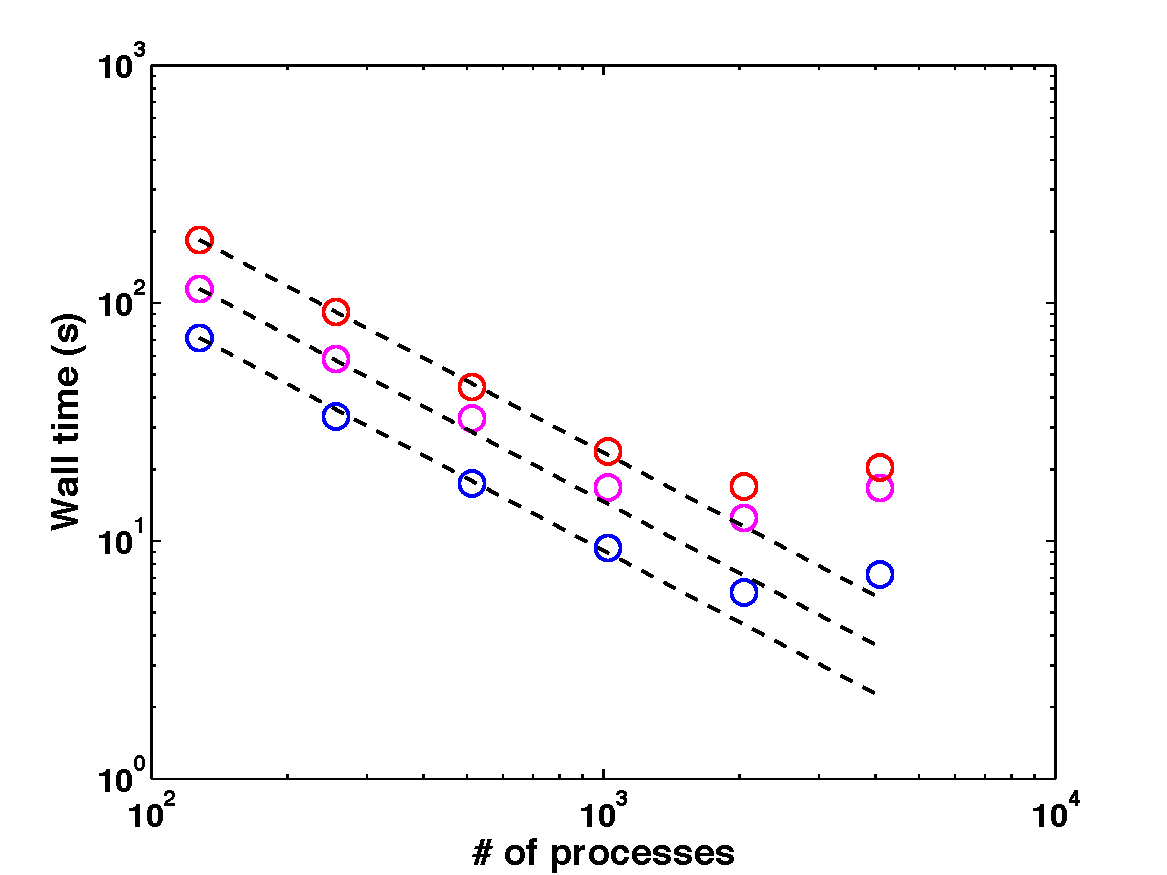
\includegraphics[width=.7\textwidth]{pictures/scaling_interpolation_all.pdf}
\caption{Scalability of the interpolation procedure. blue: alpha=0.05, purple alpha=0.50, red alpha=0.95 (alpha = percent of non-local points)}
\end{center}
\end{figure}


\subsection{Semi lagrangian advection}

\subsection{Reinitialization} \label{section::scaling_reinitialization}

The reinitialization procedure presented in section \ref{section::reinitialization} necessitates the second order derivatives of the level-set function for the second order discretization in space. The finite difference schemes we implemented rely on the description of the neighborhood of each vertex in the adaptive tree environment. This information can either be computed on the fly or stored in a buffer. Fetching the neighbors information is rather time consuming and was observed to improve the overall scalability of the algorithm by increasing the local computation load. However, it slowed down the procedure significantly and therefore we choose to present the buffered version of the implementation. If one was to be limited in memory, constructing the neighborhood information on the fly would be a desirable option and would lead to better scaling, but in our case memory is not a limiting factor.

The scaling results are presented in figure \ref{fig::scaling_reinitialization} and demonstrate satisfying scalability. Taking for reference the timing with $128$ processes, we observe efficiencies of $0.877$ with $1024$ processes, $0.763$ with $2048$ processes and $0.609$ with $4096$ processes.

\begin{figure}[ht!]
\begin{center}
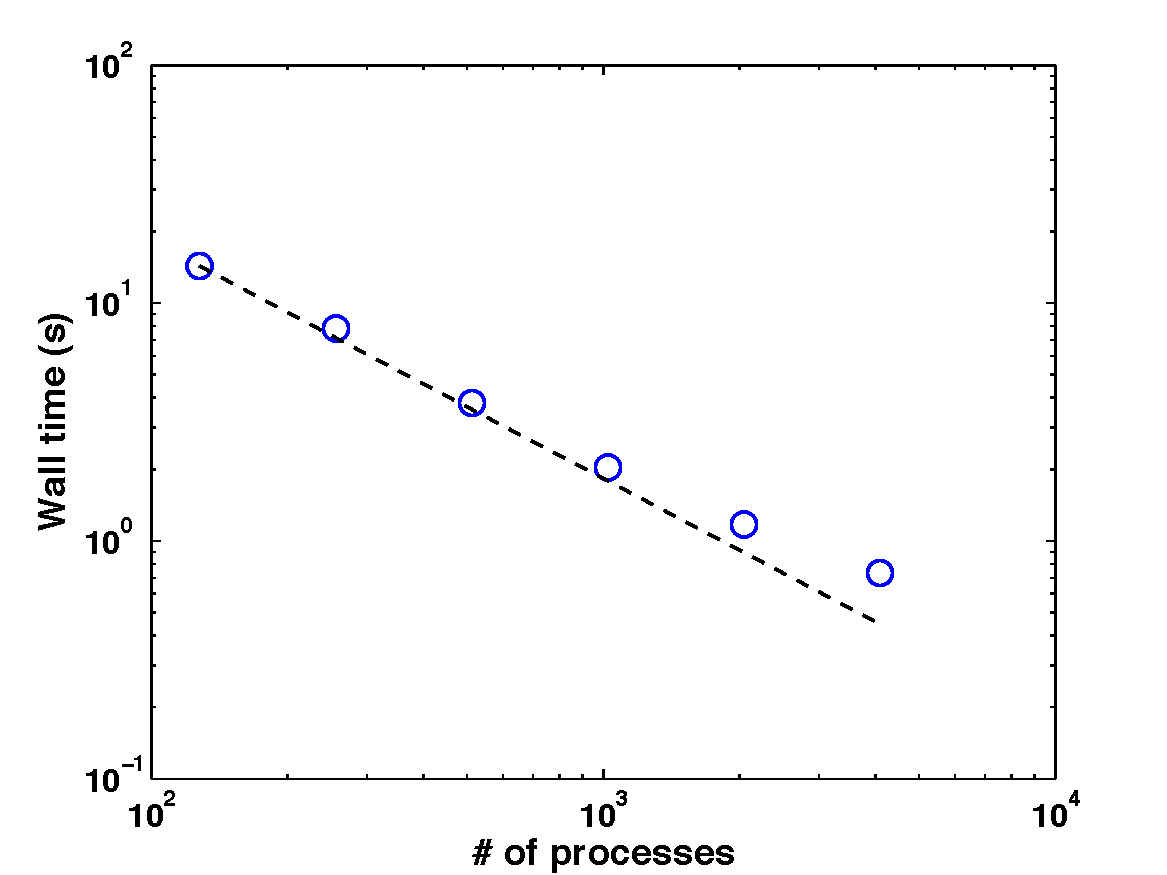
\includegraphics[width=.7\textwidth]{pictures/scaling_reinitialization_1st_time_2nd_space_with_buffer.pdf}
\caption{Scalability of the reinitialization procedure presented in section \ref{section::reinitialization} and analyzed in section \ref{section::scaling_reinitialization}.} \label{fig::scaling_reinitialization}
\end{center}
\end{figure}

\subsection{Poisson solver}